\chapter{实验四}

\section*{实验目的}

本实验（实验四）要求利用 Java 语言手工编写一个 Oberon-0 语言的递归下降预测分析程序，实现流程图自动生成。具体目标包括：

\begin{itemize}
    \item 根据 Oberon-0 的 BNF 定义设计翻译模式（Translation Scheme），将文法改造为适用于递归下降预测分析的 LL 形式。
    \item 遵循语法制导翻译的启发式规则编写递归下降预测分析程序：每非终结符对应一个递归方法，继承属性对应形式参数，综合属性对应返回值。
    \item 利用 flowchart API 自动为每个过程生成流程图——包含起始框、执行框、条件框、终止框等基本图形元素。
    \item 通过实验三（LALR 自底向上）和实验四（递归下降自顶向下）的实际体验，对两种分析策略进行全面比较。
\end{itemize}

\section*{实验目录与项目组织}

实验四的项目文件均存放于 \texttt{ex4/} 子目录下，各文件说明如下：

\begin{itemize}
    \item \texttt{src/OberonParser.java}：手工编写的递归下降预测分析程序，含翻译模式设计和流程图生成逻辑。
    \item \texttt{src/OberonScanner.java}：复用实验二由 JFlex 生成的词法分析器。
    \item \texttt{src/Token.java}、\texttt{src/exceptions/}：复用实验二的 Token 类型定义和异常类体系。
    \item \texttt{bin/}：编译后的 Java 字节码目录。
    \item \texttt{doc/}：javadoc 生成的 HTML 格式设计文档。
    \item \texttt{lib/flowchart.jar}：流程图绘制 API。
    \item \texttt{lib/jgraph.jar}：JGraph 图形库。
    \item \texttt{build.bat}、\texttt{run.bat}、\texttt{test.bat}：构建、运行和测试脚本。
\end{itemize}

\section{设计 Oberon-0 语言的翻译模式}

\subsection{文法改造}

递归下降预测分析要求文法适用于自顶向下分析，即无左递归、无公共左因子。Oberon-0 的 BNF 定义大量使用 \texttt{\{\}}（重复）和 \texttt{[]}（可选）构造，天生避免了显式左递归，无需手动消除。例如：

\begin{itemize}
    \item \path{identifier\_list = identifier \{"," identifier\}} —— 重复构造，对应循环处理。
    \item \path{statement = [assignment | procedure\_call | if\_statement | while\_statement]} —— 可选构造，对应条件判断。
    \item \path{declarations = ["CONST" \{...\}] ["TYPE" \{...\}] ["VAR" \{...\}] \{procedure\_declaration\}} —— 可选与重复的组合。
\end{itemize}

BNF 到控制流的映射规则：
\begin{itemize}
    \item \texttt{\{A\}}（重复）$\to$ \texttt{while (lookahead in FIRST(A)) \{ parseA(); \}}
    \item \texttt{[A]}（可选）$\to$ \texttt{if (lookahead in FIRST(A)) \{ parseA(); \}}
\end{itemize}

\subsection{翻译模式设计}

根据 Oberon-0 语言 BNF 定义中的语法规则，以及流程图生成的应用需求，为每个非终结符号设计对应的语义属性和翻译动作。继承属性通过 Java 方法的形式参数传递，综合属性通过返回值传递：

\begin{table}[htbp]
    \centering\small
    \begin{tabular}{|p{3cm}|p{4.5cm}|p{4.8cm}|}
    \hline
    \textbf{非终结符号} & \textbf{继承属性（输入参数）} & \textbf{综合属性（返回值）} \\
    \hline
    module & -- & -- \\
    declarations & -- & -- \\
    procedureHeading & -- & String（过程名）\\
    procedureBody & procName: String（用于 END 名称校验） & -- \\
    statement & currentBody: StatementSequence（父语句块）& -- \\
    whileStatement & currentBody: StatementSequence & -- \\
    ifStatement & currentBody: StatementSequence & -- \\
    expressionText & -- & String（表达式文本）\\
    simpleExpressionText & -- & String \\
    termText & -- & String \\
    factorText & -- & String \\
    actualParametersText & -- & String（含括号的参数文本）\\
    identifierListText & -- & String（逗号分隔的标识符列表）\\
    typeText & -- & String（类型文本）\\
    selector & -- & --（消费 Token，无返回值）\\
    \hline
    \end{tabular}
    \caption{非终结符号的翻译模式}
    \label{tab:translation-scheme}
\end{table}

\textbf{语义动作嵌入位置}（以 if\_statement 为例）：
\begin{enumerate}
    \item 匹配 IF $\to$ 向前看 Token
    \item expression() $\to$ 获取条件文本（综合属性）
    \item 语义动作：创建 \texttt{IfStatement(condition)} 对象
    \item 匹配 THEN $\to$ 将 currentBody 切换为 ifStmt.getTrueBody()，递归解析语句序列，再恢复 currentBody
    \item 匹配 ELSE $\to$ 将 currentBody 切换为 ifStmt.getFalseBody()，递归解析语句序列，再恢复 currentBody
    \item 语义动作：将 IfStatement 添加至父语句块
\end{enumerate}

\section{编写递归下降预测分析程序}

\subsection{核心方法映射}

每个非终结符号对应一个递归方法，方法命名遵循 \texttt{parseXxx()} 或 \texttt{xxxText()} 约定：

\begin{itemize}
    \item \texttt{module()} $\to$ \texttt{declarations()} $\to$ \texttt{procedureDeclaration()} $\to$ \texttt{procedureBody()}
    \item \texttt{statement()} $\to$ 根据 lookahead 类型分派到 \texttt{ifStatement()} / \texttt{whileStatement()} / assignment / procedureCall
    \item \texttt{expressionText()} $\to$ \texttt{simpleExpressionText()} $\to$ \texttt{termText()} $\to$ \texttt{factorText()}
    \item \texttt{match(Token.Type)} $\to$ 消费当前 Token 并前进；不匹配时抛出 SyntacticException
\end{itemize}

\subsection{流程图 API 集成}

在语法制导翻译过程中调用 flowchart API 构建流程图结点：

\begin{itemize}
    \item \textbf{模块}：\texttt{flowchart.Module moduleName} 创建根模块对象。
    \item \textbf{过程}：\texttt{currentModule.add(procName)} 在模块下添加过程结点，返回 Procedure 对象。
    \item \textbf{基本语句}：\texttt{currentBody.add(new PrimitiveStatement(stmtText))} 添加矩形执行框，框内显示语句文本。
    \item \textbf{IF 语句}：\texttt{new IfStatement(condition)} 创建菱形条件框；通过 \texttt{getTrueBody()} 和 \texttt{getFalseBody()} 获取真/假分支语句块，ELSIF 分支以嵌套 IfStatement 形式置于 falseBody 中。
    \item \textbf{WHILE 语句}：\texttt{new WhileStatement(condition)} 创建循环条件框；通过 \texttt{getLoopBody()} 获取循环体语句块。
\end{itemize}

\subsection{流程图生成测试结果}

利用实验一编写的测试用例对递归下降分析器进行测试：

\begin{table}[htbp]
    \centering
    \begin{tabular}{|l|c|c|l|}
    \hline
    \textbf{测试用例} & \textbf{过程数} & \textbf{流程图} & \textbf{结果} \\
    \hline
    BankSystem.obr & 8 & 完整生成 & 通过（SUCCESS）\\
    BankSystem.006 & -- & -- & SyntacticException $\checkmark$ \\
    BankSystem.007 & -- & -- & SyntacticException $\checkmark$ \\
    BankSystem.008 & -- & -- & SyntacticException $\checkmark$ \\
    BankSystem.009 & -- & -- & MissingOperandException $\checkmark$ \\
    BankSystem.010 & -- & -- & SyntacticException $\checkmark$ \\
    BankSystem.013 & 1 & 部分生成 & SemanticException $\checkmark$ \\
    \hline
    \end{tabular}
    \caption{实验四递归下降分析器测试结果汇总}
    \label{tab:parser4-results}
\end{table}

BankSystem.obr 的递归下降分析生成了 8 个过程（7 个用户声明过程 + 模块主体）的完整流程图。使用 Xvfb 虚拟显示器在服务器端渲染的流程图如图 \ref{fig:flowchart} 所示。

\begin{figure}[htbp]
    \centering
    \begin{subfigure}[b]{0.32\textwidth}
        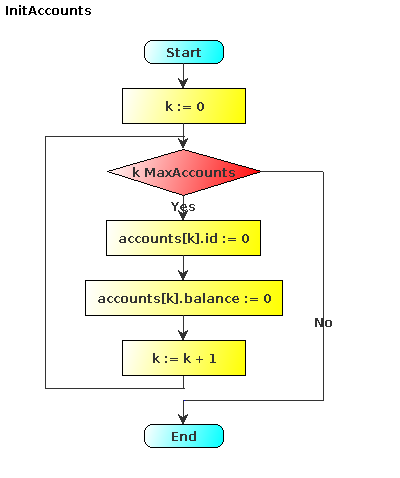
\includegraphics[width=\textwidth]{image/flowcharts/flowchart_7_InitAccounts.png}
        \caption{InitAccounts}
    \end{subfigure}
    \begin{subfigure}[b]{0.32\textwidth}
        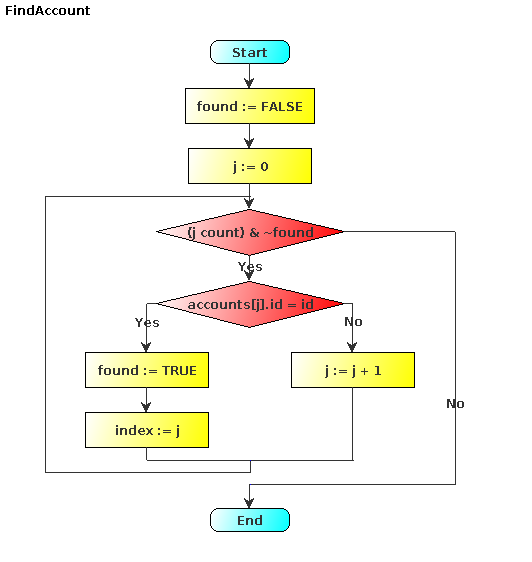
\includegraphics[width=\textwidth]{image/flowcharts/flowchart_6_FindAccount.png}
        \caption{FindAccount}
    \end{subfigure}
    \begin{subfigure}[b]{0.32\textwidth}
        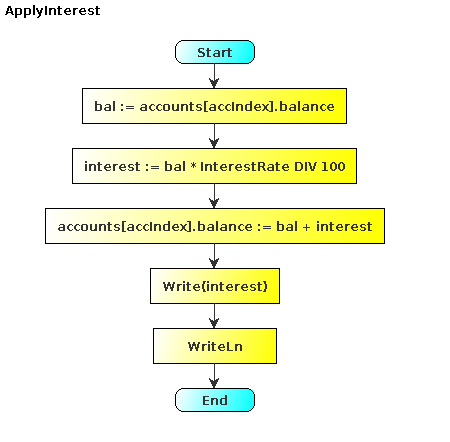
\includegraphics[width=\textwidth]{image/flowcharts/flowchart_1_ApplyInterest.png}
        \caption{ApplyInterest}
    \end{subfigure}
    \begin{subfigure}[b]{0.32\textwidth}
        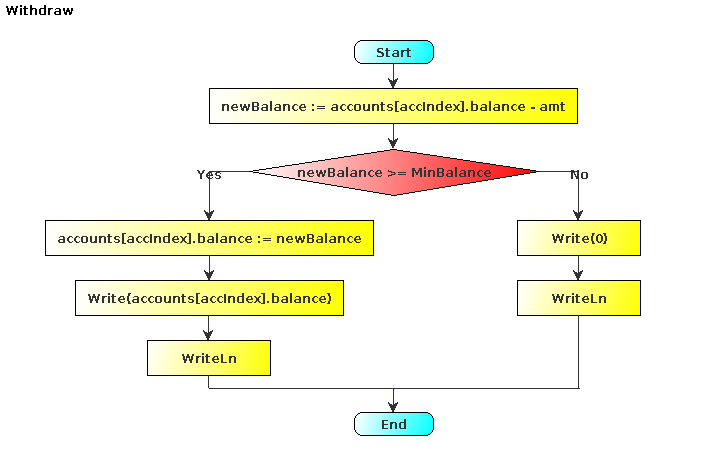
\includegraphics[width=\textwidth]{image/flowcharts/flowchart_8_Withdraw.png}
        \caption{Withdraw}
    \end{subfigure}
    \begin{subfigure}[b]{0.32\textwidth}
        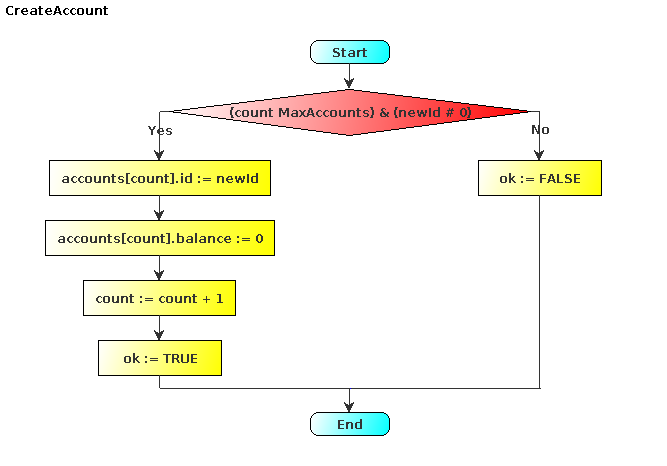
\includegraphics[width=\textwidth]{image/flowcharts/flowchart_4_CreateAccount.png}
        \caption{CreateAccount}
    \end{subfigure}
    \begin{subfigure}[b]{0.32\textwidth}
        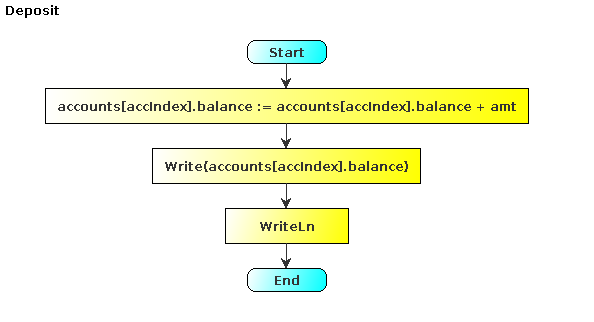
\includegraphics[width=\textwidth]{image/flowcharts/flowchart_5_Deposit.png}
        \caption{Deposit}
    \end{subfigure}
    \begin{subfigure}[b]{0.32\textwidth}
        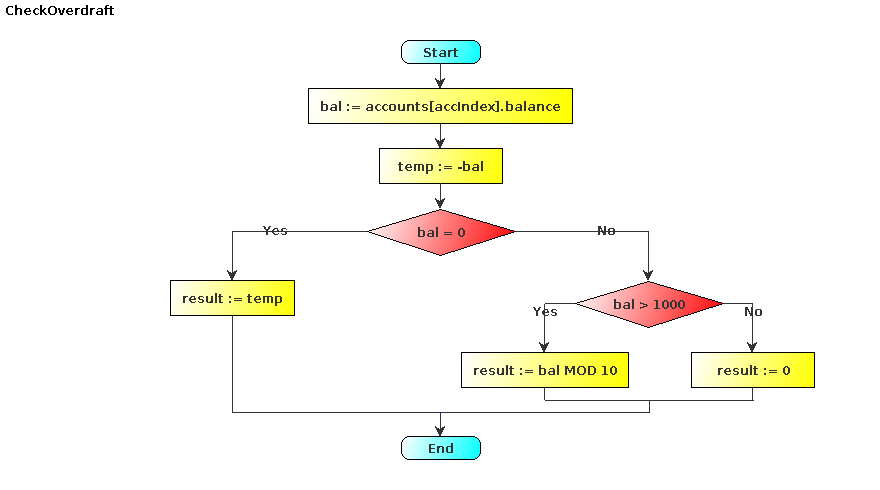
\includegraphics[width=\textwidth]{image/flowcharts/flowchart_3_CheckOverdraft.png}
        \caption{CheckOverdraft}
    \end{subfigure}
    \\[4pt]
    \begin{subfigure}[b]{\textwidth}
        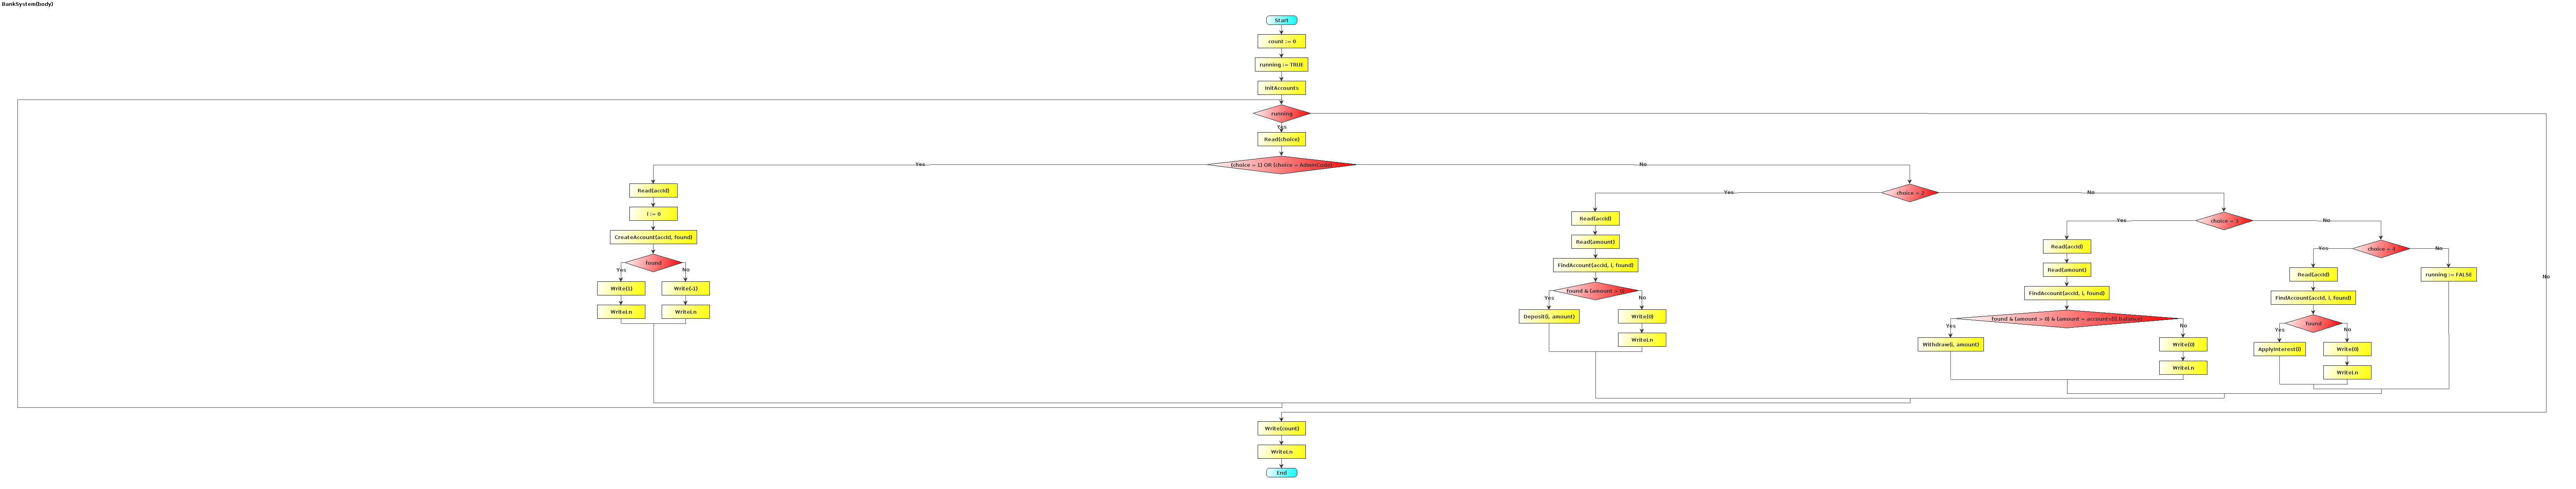
\includegraphics[width=\textwidth,height=5cm,keepaspectratio=false]{image/flowcharts/flowchart_2_BankSystem_body_.png}
        \caption{BankSystem (module body)}
    \end{subfigure}
    \caption{BankSystem.obr 经递归下降分析器生成的流程图（全部 8 个过程）}
    \label{fig:flowchart}
\end{figure}

\section{自顶向下 vs. 自底向上分析策略比较}

通过实验三（JavaCUP LALR 自底向上）和实验四（手工递归下降自顶向下）的亲身实践，对两种分析策略进行全面比较：

\begin{table}[htbp]
    \centering\small
    \begin{tabular}{|p{3cm}|p{4.5cm}|p{4.5cm}|}
    \hline
    \textbf{比较维度} & \textbf{递归下降（自顶向下）} & \textbf{LALR（自底向上）} \\
    \hline
    简单性与直观性 & 代码直接反映文法，每非终结符对应一个方法，直观易懂 & 需理解 LR 状态机、移进/归约概念，较抽象 \\
    调试难度 & 易于调试，直接在递归方法中设断点，跟踪向前看符号 & 调试需理解自动生成的分析表，错误定位困难 \\
    文法通用性 & 仅适用于 LL(k) 文法，需消除左递归和提取公因子 & 可处理更广泛文法，包括自然左递归 \\
    语义动作集成 & 继承属性=参数、综合属性=返回值，嵌入极其自然 & 归约时执行，属性通过分析栈传递 \\
    出错恢复 & 恐慌模式易于实现（跳过直到同步符号） & 需在生成框架中插入错误回调 \\
    分析表大小 & 无需显式分析表（程序结构即分析表） & LALR 表较 LR(1) 紧凑，但状态数仍较多 \\
    分析速度 & 递归调用有开销，教学语境足够 & 表驱动状态跳转通常更快 \\
    开发效率 & 手工编写代码量大，但理解深入 & 工具生成，规格文件紧凑 \\
    \hline
    \end{tabular}
    \caption{递归下降与 LALR 分析策略的全面比较}
    \label{tab:parsing-compare}
\end{table}

就本实验而言，两种方法各有所长：

\begin{itemize}
    \item \textbf{递归下降}更适合手工编写的教学场景。Oberon-0 的 BNF 使用 \texttt{\{\}} 和 \texttt{[]} 天然避免了左递归，使得文法到代码的映射极为直接。调试时可以直接在递归方法中设置断点，观察向前看符号和当前解析状态，学习曲线平缓。
    \item \textbf{LALR}更适合处理复杂文法的工业场景。JavaCUP 自动生成 190 个解析状态的 LALR 分析器，规格文件 120 行即可描述完整文法，避免了手工编写大量重复代码。工具自动检测文法冲突，生成的代码经充分测试后可靠性更高。
\end{itemize}

Oberon-0 的 BNF 设计对两种方法均十分友好：其 \texttt{\{\}}/\texttt{[]} 构造天然消除左递归适合递归下降，同时文法层次清晰、无二义性也适合 LALR 分析。这体现了 Wirth 对语言简洁性和分析友好性的追求。

\section{自我评分参照}

参照实验四评价标准，各项完成情况如下：

\begin{table}[htbp]
    \centering
    \begin{tabular}{|p{4.5cm}|c|c|p{4.5cm}|}
    \hline
    \textbf{项目} & \textbf{权重(\%)} & \textbf{对应内容} \\
    \hline
    1、Oberon-0 语言的翻译模式 & 30  & 4.1节 翻译模式设计 + 表 \\
    2、语法分析程序源代码 & 40  & 4.2节 OberonParser.java \\
    3、程序运行与测试 & 15  & 4.3节 8过程流程图 + 错误检测 \\
    4、面向对象设计与编码风格 & 10  & 流程图API 组合模式 \\
    5、文档组织及 readme 等 & 5  & ex4/readme.txt + 脚本 + javadoc \\
    \hline
    \end{tabular}
    \caption{实验四自我评分参照}
    \label{tab:self-eval-ex4}
\end{table}

\section{实验心得体会}

实验四的手工递归下降分析器编写是我在编译原理课程中最有收获的一次实践。与实验三使用 JavaCUP 自动生成分析器的"声明式"体验不同，手工编写递归下降代码让我对语法分析的每一处细节——从向前看符号的判断到语义动作的嵌入时机——都有了切身的理解。

翻译模式的设计是本次实验的核心挑战。将 BNF 产生式映射为递归方法看似机械，但实际编码中需要仔细处理多个细节：(1) 继承属性的传递方向——IF 语句需要将父语句块的引用传递给分支解析；(2) ELSIF 链的嵌套表示——每个 ELSIF 在流程图中成为前一个 IfStatement 的 falseBody 中的新的 IfStatement；(3) 表达式文本的综合属性收集——多级运算符优先级要求每级方法正确拼接子表达式的文本。

将流程图 API 集成到递归下降分析器中的过程，让我深刻体会到语法制导翻译中"语义动作嵌入"的优雅——在解析 IF 关键字后立即创建 IfStatement 对象，在 THEN 后将解析上下文切换到 trueBody，在 ELSE 后切换到 falseBody，在 END 后将完整的 IfStatement 添加回父语句块。这种"解析到哪、构造到哪"的即时翻译方式，远比解析完成后遍历 AST 的后处理方式直观。

与实验三的对比让我对自顶向下和自底向上两种分析策略有了更平衡的认识。递归下降在可调试性和语义动作集成方面有明显优势，但 LALR 在文法通用性和开发效率上更胜一筹。实践中，C 语言家族的工业级编译器（GCC、Clang）普遍采用手工递归下降，这既是因为 C 的文法不适合纯 LR 分析（需要"lexer hack"来处理类型名与变量名的歧义），也是因为手工编写更便于生成高质量的错误信息——这一点在本次实验中也有切身体会。
